\documentclass{article}
\usepackage{fullpage,amsmath,amsthm,graphicx,enumitem,amssymb}
\usepackage[hidelinks]{hyperref}
\usepackage{todonotes}
\theoremstyle{definition}
\newtheorem{thm}{Theorem}
\newtheorem{question}[thm]{Question}
\newenvironment{solution}{\noindent\textit{Solution:}}{}

\newcommand{\reals}{\mathbb{R}}

\title{ASEN 5264 Decision Making under Uncertainty\\
       Homework 2: Markov Decision Processes}

\begin{document}

\maketitle

\section{Conceptual Questions}

\begin{question} (10 pts)
    \begin{enumerate}[label=\alph*)]
        \item Describe the difference between the reward function and the state-action ($Q$) value function.
        \item Write down an equation for the state-action value in terms of $R$, $T$, and $V$.
    \end{enumerate}
\end{question}

% \begin{question} (5 pts)
%     Consider the following MDP state spaces. Write down an example of a state in the specified state space. Use parentheses when the state is represented by more than one variable.
%     \begin{enumerate}[label=\alph*)]
%         \item $\mathcal{S} = \{1, 14, 37\}$
%         \item $\mathcal{S} = [-1, 2]$ (the closed interval between -1 and 2)
%         \item $\mathcal{S} = [0, 2] \times [-2, 0]$
%         \item $\mathcal{S} = \mathbbb{R}^4$
%         \item $\mathcal{S} = \mathbbb{R} \times \{a, b, c\}$
%     \end{enumerate}
% \end{question}

\begin{question} (25 pts)
    Consider a game with 3 squares in a horizontal line drawn on paper, a token, and a die. Each turn, the player can either reset or roll the die. If the player rolls and the die shows an odd number, the token is moved one square to the right, and if an even number is rolled, the token is moved two squares to the right (in both cases stopping at the rightmost square\footnote{If the die is rolled from the middle square or right square, it will always end up in the right square.}). If the player resets, the token is always moved to the leftmost square. If the reset occurs when the token is in the middle square, two points are added; if the player resets when the token is on the right square, a point is subtracted.
    \begin{enumerate}[label=\alph*)]
        \item Formulate this problem as an MDP (write down $S$, $A$, $T$, and $R$).
        \item Calculate the optimal value when the token is in the leftmost square assuming a discount factor of $\gamma = 0.95$.\footnote{Hint: Guess an optimal policy, evaluate that optimal policy, and then verify that it satisfies the Bellman equation.}
        \item Suppose you are not sure that the die is fair (i.e. whether it will yield odd and even with equal probability). Give finite upper and lower bounds for the accumulated discounted score that you can expect to receive with discount $\gamma = 0.95$.
    \end{enumerate}
\end{question}

\section{Exercise}

\begin{question} \label{q:gw}
    (Value iteration for Grid World, 35 pts)

    Solve the MDP \texttt{HW2.grid\_world} with your own implementation of value iteration with a discount of $\gamma=0.95$ and plot the resulting value function. All of the necessary information to solve this problem can be extracted with the \texttt{HW2.transition\_matrices} and \texttt{HW2.reward\_vectors} functions, and plotting can be accomplished with \texttt{POMDPModelTools.render(HW2.grid\_world, color=v)} where \texttt{v} is the value function. See the starter code and function docstrings for more information.
\end{question}

\section{Challenge Problem}

\begin{question}
    (Value iteration for ACAS, 20 pts autograder, 10 pts code)

Your task is to find the optimal value function for an Aircraft Collision Avoidance System (ACAS). The encounter model will be specified as a Markov decision process, and your task will be to compute the value function for discount $\gamma=0.99$ using value iteration or another suitable algorithm that you implement. The continuous physical state space will be discretized at various levels of granularity and the goal is to find the value function for the finest discretization possible.

A model with discretization level \texttt{n} can be constructed with
\begin{verbatim}
                        m = HW2.UnresponsiveACASMDP(n)
\end{verbatim}
The higher \texttt{n} is, the finer the discretization and the larger the state space. Again, all of the information needed to solve this problem can be extracted with the \texttt{HW2.transition\_matrices} and \texttt{HW2.reward\_vectors} functions, so you can start with your code from Question \ref{q:gw}.

The score received for solving the problem is \texttt{n}. You must submit your code for this problem along with the \texttt{results.json} file from executing \texttt{HW2.evaluate(v, "email@colorado.edu")} where \texttt{v} is the value function vector\footnote{\texttt{HW2.evaluate} will check the value function with a tolerance of $1 \times 10^{-6}$}. A score of \texttt{n} = 7 or higher will receive full credit\footnote{By taking advantage of the structure of the problem, it is possible to attain a score of \texttt{n} = 20 with less than 10 minutes of computation time on a single core of a i7 laptop processor.}.

\vspace{1em}
\noindent\makebox[\linewidth]{\rule{\textwidth}{0.4pt}}
\vspace{1em}

\textbf{The information above this line is sufficient to complete this homework and receive full credit.} However, the description of the model below may help to get the highest score on the leaderboard. The \texttt{UnresponsiveACASMDP} model implements the POMDPs.jl explicit MDP interface\footnote{The \texttt{states}, \texttt{actions}, \texttt{reward}, and \texttt{transition} functions from POMDPs.jl.}, and students are welcome to explore the problem further using that interface as well as ask on Ed and look at the source code for details. The underlying continuous model is defined as follows:

\begin{center}
    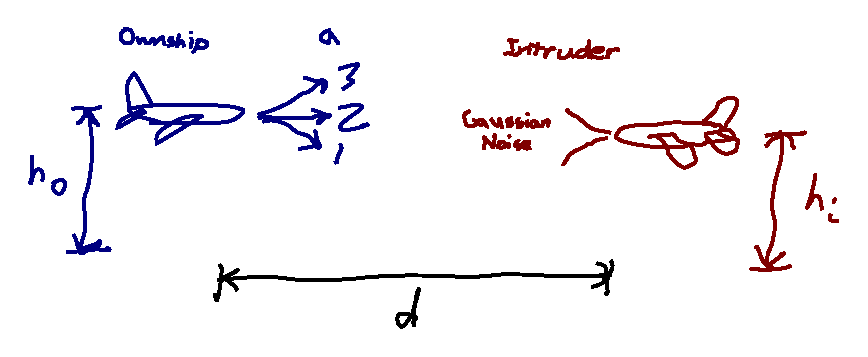
\includegraphics[width=0.7\textwidth]{unresponsive_acas.pdf}
\end{center}

\begin{itemize}
    \item The state space is 4-dimensional $\mathcal{S} = \reals^4$, with each state consisting of $s=(h_o, \dot{h}_o, h_i, d)$ where $h_o$ is the ownship altitude in feet, $\dot{h}_o$ is the rate of climb in ft/min, $h_i$ is the intruder altitude in feet, and $d$ is the distance between the aircraft in feet.
    \item The action space is $\mathcal{A}=\{-1500, 0, 1500\}$ and represents the change in rate of climb. The possible rates of climb are $\dot{h}_o \in \{-3000, -1500, 0, 1500, 3000\}$
    \item A reward of -100 is received for a near-mid-air collision, defined as the aircraft passing within 500 vertical feet and 100 horizontal feet of each other. Any change in rate of climb yields a reward of -1.
    \item The rate of climb, $\dot{h}_o$ changes instantly when an action is applied. Then the following dynamics are used: $d' = d - 2\,v\,\Delta t$ where $v$ is the fixed horizontal velocity, $h_o' = h_o + \dot{h}_o\,\Delta t$, and $h_i' = h_i + W_{\Delta t \sigma^2}$ where $W$ is the Wiener process\footnote{\url{https://en.wikipedia.org/wiki/Wiener_process}}. $\Delta t$ changes based on the discretization \texttt{n}.
\end{itemize}

\end{question}

\end{document}
